%\graphicspath{{~/Pictures/Screenshots/}}
\graphicspath{{~/Documents/MobAppDev/SecondTask/PNG}}
\section*{\LARGE{Цель практической работы}}
\addcontentsline{toc}{section}{Цель практической работы}
В практической работе была рассмотренно как использовать базовые возможности
платформы для управления ресурсами для оптимизации приложения
под различные Android-совместимые устройства, и разместить его в
единственном APK-файле.

\newpage

\section*{\LARGE{Выполнение практической работы}}
\addcontentsline{toc}{section}{Выполнение практической работы}

\section{Поддержка различных языков}
Размещение строковых констант в отдельном файле считается хорошим
тоном. В каждом проекте Andoid для строковых констант существует
специальная директория.\par
Когда создются проекты используя инструменты Android SDK, то
директория \texttt{res/} создается автоматически в корневой директории
проекта. Также для каждого из типов ресурсов создаются собственные
поддиректории, а так же несколько стандартных файлов. Например
файл \texttt{res/values/strings.xml}, в котором хранятся строковые константы.

\subsection{Создание директорий для поддержки различных языков}
Для поддержки нескольких языков, необходимо создать в директории res
несколько дополнительных директорий values, содержащих в имени ISO
коды языков. К примеру, директория values-ru будет включать в себя ресурсы
для поддержки русского языка.
Android загружает нужные ресурсы в соответствии с настройками
локализации устройства, на котором было запущено приложение.
Чтобы включить поддержку нескольких языков, создали
необходимые поддиректории и файлы строковых ресурсов. К примеру, как
на рисунке \ref{fig:res:values}.

\begin{figure}[h!tp]
	\centering
	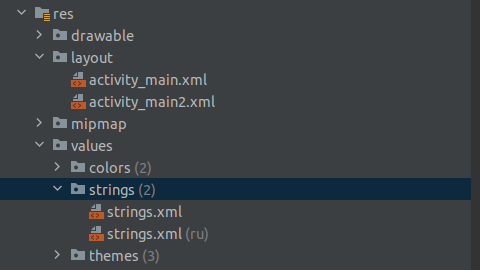
\includegraphics[width=0.8\textwidth]{Screenshot from 2023-02-20 18-03-12.png}
	\caption{Директория ресурсов проекта}
	\label{fig:res:values}
\end{figure}

Добавили строковые константы в каждый из файлов.\par
При запуске Android самостоятельно выберет подходящий файл в
соответствии с настройками локализации устройства.\par
Пример содержания файлов строковых ресурсов для различных
языков:
\begin{itemize}
	\item Английский (по умолчанию), /values/strings.xml,
		рисунок~\ref{fig:res:values:en}.
		\begin{figure}[h!tp]
			\centering
			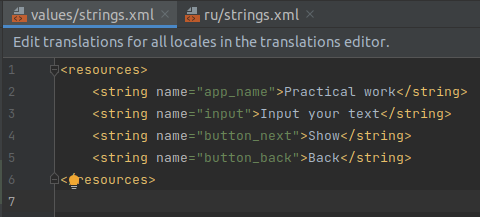
\includegraphics[width=0.7\textwidth]{Screenshot from 2023-02-20 18-13-18.png}
			\caption{Файл английских ресурсов}
			\label{fig:res:values:en}
		\end{figure}
	\item Русский, /values-ru/strings.xml,
		рисунок~\ref{fig:res:values:ru}.
		\begin{figure}[h!tp]
			\centering
			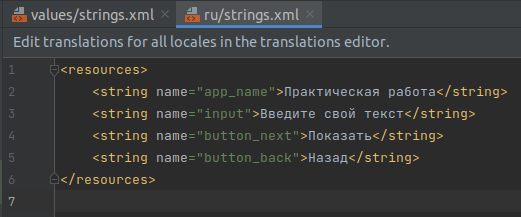
\includegraphics[width=0.7\textwidth]{Screenshot from 2023-02-20 18-13-33.png}
			\caption{Файл русских ресурсов}
			\label{fig:res:values:ru}
		\end{figure}
\end{itemize}

\subsection{Использование строковых ресурсов}
Можно ссылаться на строковые ресурсы из программного кода и других
XML файлов, используя название ресурса, которое задается в свойстве name
элемента \texttt{<string>}.\par
На строковый ресурс можно ссылаться из XML файлов разметки,
используя синтаксис \texttt{@string/<string\_name>}, всякий раз,
когда требуется строковое значение для свойства, как показано
на рисунке~\ref{fig:xml:string}.
\begin{figure}[h!tp]
	\centering
	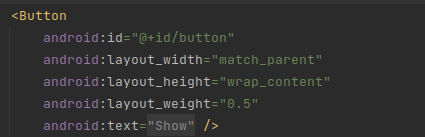
\includegraphics[width=0.8\textwidth]{Screenshot from 2023-02-20 18-33-17.png}
	\caption{Использование ресурсов в xml файле}
	\label{fig:xml:string}
\end{figure}

\section{Поддержка устройств с различными экранами}
Экраны Android устройств различаются по двум основным параметрам:
размер и разрешение. Это значит, что приложение
может быть установлено на устройствах с различными размерами и
разрешениями экрана. Чтобы оптимизировать приложение под различные
размеры и разрешения, оно должно содержать разные ресурсы под каждый
вид экрана.

\begin{itemize}
	\item Существует четыре обобщенных размера: маленький (small),
		нормальный(normal), большой(large), очень большой(x-large).
	\item Также существует четыре вида разрешений: низкое (low), среднее
		(mdpi), высокое (hdpi), очень высокое (xhdpi).
\end{itemize}

Чтобы использовать разную разметку и изображения для разных экранов,
необходимо размещать данные ресурсы в различные директории, точно
также, как мы это делали со строками для различных языков.\par
Также следует помнить об ориентации экрана (альбомная (landscape) или
портретная (portrait)), она так же считается отдельным размером и для
многих приложений необходимо отдельно оптимизировать разметку для
двух ориентаций.

\subsection{Создание различной разметки}
Чтобы оптимизировать пользовательский интерфейс под различные размеры
экрана, необходимо создать собственные файлы разметки для каждого из
размеров, которые вы хотите поддерживать. Каждый файл разметки должен
быть сохранен в соответствующей директории, название которой
заканчивается строкой \texttt{<screen\_size>}. Например, файл разметки для
больших экранов должен быть сохранен в директории \texttt{res/layout-large/}.

Директория проекта, который включает в себя стандартную разметку и разметку
для больших экранов, показан на рисунку \ref{fig:res:layout}.
\begin{figure}[h!tp]
	\centering
	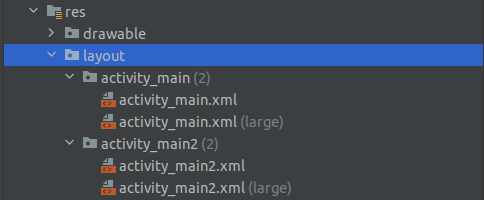
\includegraphics[width=0.8\textwidth]{Screenshot from 2023-02-20 19-31-44.png}
	\caption{Разметка для разный размеров экрана}
	\label{fig:res:layout}
\end{figure}

\section{Использование различных изображений}
Растровые изображения нужно создавать для каждого из основных
разрешений: низкого, среднего, высокого и очень высокого. Это позволит
добиться отличного качества и производительности на устройствах с любым
разрешением.\par
Чтобы создать такие изображения, создали базовый вариант в векторном
формате, а затем экспортировали его в растровый формат для каждого
разрешения, используя следующую шкалу размеров:

\begin{itemize}
	\item xhdpi: 2.0
	\item hdpi: 1.5
	\item mdpi: 1.0 (базовый размер)
	\item ldpi: 0.75
\end{itemize}

Это означает, что если создали картинку размером 200×200 пикселей для
xhdpi устройств, то для остальных устройств будут такие размеры: 150x150
для hdpi, 100×100 для mdpi и 75x75 для ldpi устройств.
После этого разместили файлы в соответствующих директориях, как показано
на рисунке~\ref{fig:res:drawable}.
\begin{figure}[h!tp]
	\centering
	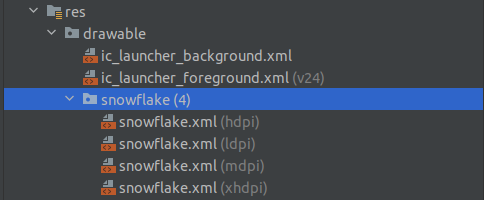
\includegraphics[width=0.8\textwidth]{Screenshot from 2023-02-20 20-10-08.png}
	\caption{Разметка для разный размеров экрана}
	\label{fig:res:drawable}
\end{figure}

\section{Поддержка различных версий Android}
В то время, как последние версии Andoid часто добавляют в API
великолепные возможности, вы должны продолжать поддерживать старые
версии Android до тех пор, пока большинство устройств не получат
обновление. В этом уроке мы рассмотрим как используя широкие
возможности последних API также продолжать поддержку старых версий
Android.\par
Диаграмма используемых версий регулярно обновляется и показывает
соотношение установленных версий Android. Диаграмма строится на основе
статистики из Google Play Store. В целом, хорошей практикой является
поддержка 90\% активных устройств при нацеливании на последние версии.

\subsection{Указание минимальной и целевой версии API}
В файле \texttt{AndroidManifest.xml} описывается какие версии Android
поддерживает приложение. Конкретно указываются атрибуты
\texttt{minSdkVersion} и \texttt{targetSdkVersion} для
элемента \texttt{<uses-sdk>}, которые указывают на минималную версию
с которым ваше приложение совместимо и максимальную версию,
на которой вы разрабатывали и тестировали приложение
(Рисунок~\ref{fig:manifest}).
\begin{figure}[h!tp]
	\centering
	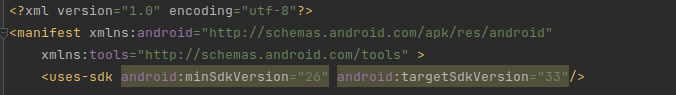
\includegraphics[width=0.8\textwidth]{Screenshot from 2023-02-20 20-20-10.png}
	\caption{Разметка для разный размеров экрана}
	\label{fig:manifest}
\end{figure}

\subsection{Получение версии Android во время выполнения приложения}
Android хранит специальный код для каждой из версий в виде константы в
классе Build.\par
В коде, изображенном на рисунке \ref{fig:code:vsdk} задает условие,
чтобы функции, доступные в более высоких версиях API выполнялись,
только если данный API доступен на устройстве.
\begin{figure}[h!tp]
	\centering
	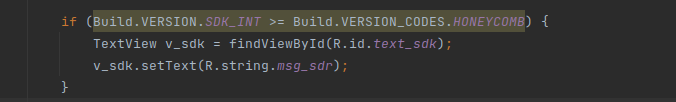
\includegraphics[width=0.8\textwidth]{Screenshot from 2023-02-20 20-37-17.png}
	\caption{Проверка версии SDK}
	\label{fig:code:vsdk}
\end{figure}

\section{Использование встроенных тем и стилей}
Android содержит стандартные темы интерфейса, которые позволяют
приложению выглядеть как одно целое с системой. Эти темы легко
использовать в приложении, указав их в файле манифеста. При
использовании встроенных тем, приложение будет «следить за модой» и
выглядеть по новому с каждым новым выпуском Android.\par
Пример, в котором явлению устанавливается ночная тема,
показан на рисунке~\ref{fig:manifest:theme}.
\begin{figure}[h!tp]
	\centering
	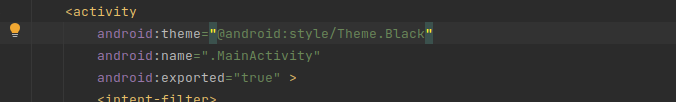
\includegraphics[width=0.8\textwidth]{Screenshot from 2023-02-20 21-00-16.png}
	\caption{Устанавливаем тему активити}
	\label{fig:manifest:theme}
\end{figure}
